\section{Controller}

\subsection{A kinematic model for the car}
The first thing to take control of a system is to understand how it
works. That's what we're going to do for this car. Indeed to control
it we will have to establish these equations in order to elaborate
the commands which will be used to lead the robot. \textbf{Figure}~\ref{fig:state}
shows the cinematic equations of the car.

\begin{figure}[!ht]
    \centering
    \begin{subfigure}[b]{0.45\textwidth}
        \centering
        
            $$ f(x, u) = \left \{
            \begin{array}{c @{=} l}
                \dot{x_1}\ & \ x_4.cos(x_5) cos(x_3) \\
                \dot{x_2}\ & \ x_4.cos(x_5) sin(x_3) \\
                \dot{x_3}\ & \ \frac{x_4 sin(x_5)}{L} \\
                \dot{x_4}\ & \ u_1 \\
                \dot{x_5}\ & \ u_2 
            \end{array}
            \right. $$
        
        \caption{Equation of the car}
        \label{eqn:state}
    \end{subfigure}
    \hfill
    \begin{subfigure}[b]{0.45\textwidth}
        \centering
        \includegraphics[width=\textwidth]{Images/state_diagram.png}
        \caption{Diagram of the car}
        \label{fig:raspi_config}
    \end{subfigure}
    \caption{State equation of the car}
    \label{fig:state}
\end{figure}



In these equations $x_1$ and $x_2$ are respectively the x and y
coordinates of the robot, $x_3$ is the heading of the robot, $x_4$
represent the speed of the rear motor and $x_5$ is the steering angle
of the car controlled by the front servomotor. $L$ is the distance between
the front and the back driving shafts. In this system it is
important to identify the variables of interest. These are the variables
that we will want to control. In our case we will be interested in the 
speed of the car and its heading.

There is a usefully tool to use when you want to understand
how to run a system from state equations. The differential delay
graph allows you to relate the inputs to the outputs of the car.
Actually each new node represents an integration of the previous variable. There is also the link between
inputs and outputs of our system. \textbf{Figure}~\ref{fig:diff_delay}
is the differential delay graph for our car. On this graph we represented
the two variables of interest with a double circle.

\begin{figure}[!ht]
    \centering
    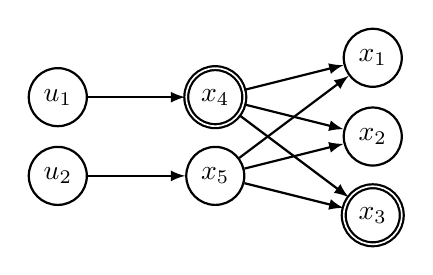
\begin{tikzpicture}[thick, scale=1, every node/.style={transform shape}]
        \tikzstyle{n}=[circle,draw]
        \tikzstyle{dn}=[circle, draw, double]
        \node[n] (U1) at (0,1) {$u_1$};
        \node[n] (U2) at (0,0) {$u_2$};
        \node[dn] (X4) at (2,1) {$x_4$};
        \node[n] (X5) at (2,0) {$x_5$};
        \node[n] (X1) at (4,1.5) {$x_1$};
        \node[n] (X2) at (4,0.5) {$x_2$};
        \node[dn] (X3) at (4,-0.5) {$x_3$};

        \tikzstyle{late}=[->,>=latex]
        \draw[late] (U1)--(X4);
        \draw[late] (U2)--(X5);
        \draw[late] (X4)--(X1);
        \draw[late] (X4)--(X2);
        \draw[late] (X4)--(X3);
        \draw[late] (X5)--(X1);
        \draw[late] (X5)--(X2);
        \draw[late] (X5)--(X3);
    \end{tikzpicture}
    \caption{Differential delay graph of our car}
    \label{fig:diff_delay}
\end{figure}


As we can see on the differential delay graph shown on \textbf{Figure}~\ref{fig:diff_delay},
there is only one integration between the inputs and the $x_4$ output against a
minimum of two integrations between the inputs and the $x_3$ output. We will therefore
be able to act faster on the speed of the car than on its heading. Moreover we
notice that to change the orientation of the car, we need both inputs. Indeed,
the orientation of the front direction has no effect on the orientation of the
car if it is motionless.

\subsection{Simple law of control}

In the case of a system that was originally built to be driven by a human, reference
\cite{robmooc} tells us that it is possible to develop simple controls that would
imitate the behaviour of a human pilot. Indeed, by following thetwo principles stated below,
it is possible to take control of the car in a very simplistic but at least functional way.

\begin{itemize}
    \item \textbf{First principles} The speed of the car must be constant and not null.
    \item \textbf{Second principles} The further the car is from the target, the more the car will turn.
\end{itemize}

With the first principle, we ensure that the car will run at all times, and therefore that
the action on the steering will allow the car's heading to be adjusted. The second principle
simply indicates that the further the car moves to the right of the line, the more it will 
turn to the left and vice versa. Thus the car will tend to return closer to the line.

According to reference 2, it is necessary to take the arctangent of the error in order to
have a saturation effect on the control. The error here is of course the distance between
the center of the car and the center of the line. We have chosen the arctangent shown in
\textbf{Figure}~\ref{fig:arctan}. With this function, we are sure that the order law will
not diverge, even if the line is far from the center of the picture.

\begin{figure}[!ht]
    \begin{center}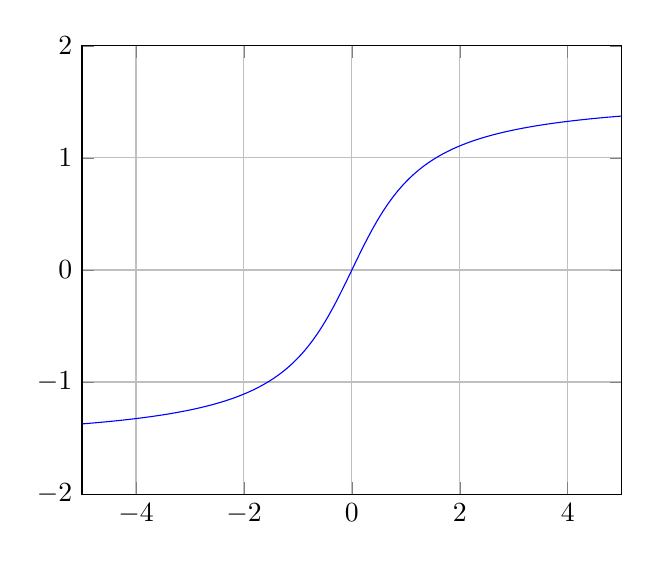
\begin{tikzpicture}
        \begin{axis}[xmin=-5, xmax=5, ymin=-2, ymax=2, samples=50, grid=both]
            \addplot[mark=none,color=blue, samples=500]{rad(atan(x))};
          \end{axis}
    \end{tikzpicture}\end{center}
    \caption{Arctan control saturation for car steering}
    \label{fig:arctan}
\end{figure}

In conclusion, noting $e$ the error and $v_0$ the desired speed which will be constant,
this simple control law will come from the equations~\ref{eqn:simple_law}.

\begin{equation}
    \label{eqn:simple_law}
    \left\{
        \begin{array}{c @{=} l}
            u_1\ & \ v_0 \\
            u_2\ & \ arctan(e)
        \end{array}
    \right. 
\end{equation}

% Maybe a future part

% \subsection{Guidance of the car}
% The control law of the previous section is very effective in case the line is visible
% by the car. However, there may be cases where the car has moved away from this line.
% The requirement XXXXXXXXXXX in the requirements diagram tells us that the car must be
% able to make the turn even if the car has deviated slightly from the line. The car will
% be able to use virtual GPS markers that will be placed along the route to guide it back
% and forth along the line. This control law should be seen as something more advanced,
% which will allow the system to truly achieve its mission.

\newpage